\chapter{हाइड्रोजन और s-ब्लॉक}\label{ch:b1:s-block}

हर फ़ोन, लैपटॉप और इलेक्ट्रिक कार में एक बैटरी होती है जिसके धन
आवेश लिथियम आयन ढोते हैं। वह लिथियम मुख्यतः दो
स्थानों से आता है: ऑस्ट्रेलिया की कठोर-चट्टान खानें और एंडीज़ के लवण-मैदान, जहाँ
भू-पर्पटी के नीचे से पंप किया गया लवण-जल महीनों तक धूप में वाष्पित होने के लिए छोड़ दिया जाता है,
जब तक उससे लिथियम लवण अवक्षेपित न किए जा सकें। लिथियम \omterm{def:b1:s-block:families}{क्षार धातुओं} में पहला है,
जो सबसे अधिक अभिक्रियाशील धातुएँ हैं, और उसके पड़ोसी सोडियम, पोटैशियम, मैग्नीशियम और कैल्सियम
उद्योग के थोक रसायन देते हैं: कॉस्टिक सोडा, सोडा ऐश, चूना। यह अध्याय
हाइड्रोजन और \omterm{def:b1:periodicity:table}{s-ब्लॉक} के साथ तत्त्वों के वर्णनात्मक रसायन का आरंभ करता है,
और पिछले अध्यायों के उपकरणों --- आयनन ऊर्जाओं,
\omterm{def:b1:nernst:electrode-potential}{मानक विभवों}, \omterm{def:b1:precipitation:solubility-product}{विलेयता गुणनफलों} --- से यह समझाता है कि ये
तत्त्व क्या करते हैं।

\begin{recall}
आयनन ऊर्जाएँ और \omterm{def:b1:periodicity:electronegativity}{विद्युत-ऋणात्मकता} (\cref{ch:b1:periodicity});
\omterm{def:b1:nernst:electrode-potential}{मानक विभव} (\cref{ch:b1:nernst}); \omterm{def:b1:precipitation:solubility-product}{विलेयता गुणनफल} और
हाइड्रॉक्साइडों का अवक्षेपण (\cref{ch:b1:precipitation})। विद्यालय के
खंड (कक्षा 10) ने तत्त्वों को कुलों में समूहित किया था: \omterm{def:b1:s-block:families}{क्षार धातुएँ},
\omterm{def:b1:s-block:families}{क्षारीय मृदा धातुएँ}, हैलोजन, उत्कृष्ट गैसें।
\end{recall}

\begin{omfigure}
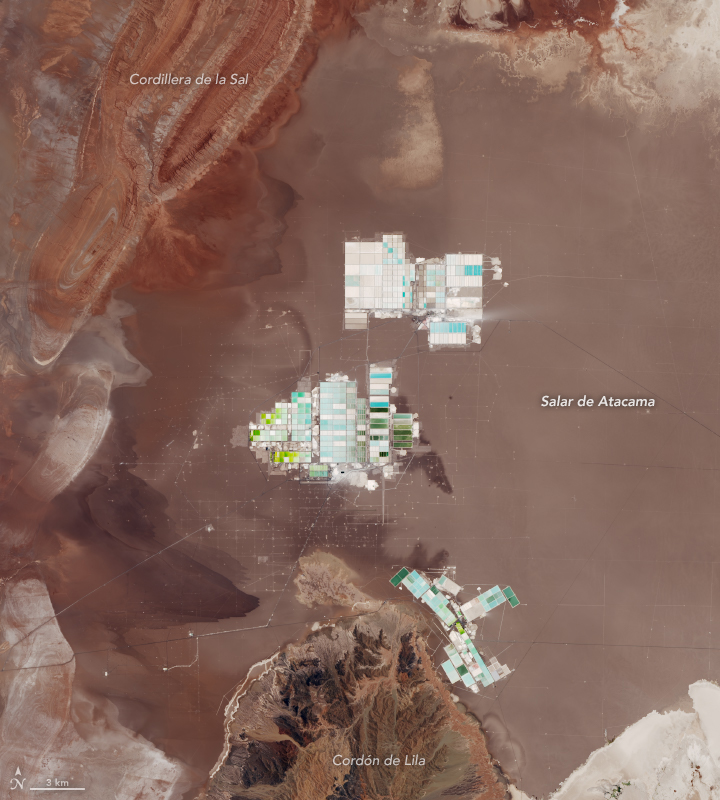
\includegraphics[width=0.48\linewidth]{images/book2/atacama-ponds.jpg}

{\small सालार दे अटाकामा पर लिथियम लवण-जल के वाष्पन तालाब, कक्षा से
देखे गए (लैंडसैट 8, 2018; नासा अर्थ ऑब्ज़र्वेटरी, सार्वजनिक अधिकार-क्षेत्र,
विकिमीडिया कॉमन्स)। लवण-जल के सांद्र होने और लवणों के क्रिस्टलित होने के साथ
हर तालाब का रंग बदलता है।}
\end{omfigure}

\section{हाइड्रोजन और हाइड्राइड}

हाइड्रोजन के पास एक इलेक्ट्रॉन है: वह उसे खो सकता है (\ce{H+}, जिसे जल
\ce{H3O+} के रूप में ढोता है), साझा कर सकता है (\omterm{def:b1:lewis-resonance-vsepr:lewis}{सहसंयोजी आबंध}), या एक प्राप्त कर सकता है (\ce{H-}, हीलियम के
\omterm{def:b1:quantum-numbers:configuration}{इलेक्ट्रॉनिक विन्यास} के साथ)। वह इनमें से क्या करता है, यह उसके भागीदार पर निर्भर करता है।

\begin{definition}[हाइड्राइड]\label{def:b1:s-block:hydride}
\emph{हाइड्राइड}\index{हाइड्राइड} किसी अन्य तत्त्व के साथ हाइड्रोजन का
द्विअंगी यौगिक है। \emph{लवणीय हाइड्राइड}\index{लवणीय हाइड्राइड}, जो
\omterm{def:b1:s-block:families}{क्षार धातुओं} और भारी \omterm{def:b1:s-block:families}{क्षारीय मृदा धातुओं} के साथ बनते हैं (\ce{LiH}, \ce{NaH},
\ce{CaH2}), \ce{H-} युक्त आयनिक ठोस हैं। \emph{सहसंयोजी
हाइड्राइड}\index{सहसंयोजी हाइड्राइड}, जो \omterm{def:b1:periodicity:table}{p-ब्लॉक} तत्त्वों के साथ बनते हैं
(\ce{CH4}, \ce{NH3}, \ce{H2O}, \ce{HCl}), आण्विक हैं। \emph{धात्विक
हाइड्राइड}\index{धात्विक हाइड्राइड}, जो कुछ संक्रमण धातुओं के साथ बनते हैं,
ऐसे ठोस हैं जिनमें हाइड्रोजन धातु \omterm{def:b1:crystals-metals:lattice}{जालक} के \omterm{def:b1:crystals-metals:site}{अंतराकाशी स्थल} घेरता है, प्रायः
परिवर्ती संघटन के साथ।
\end{definition}

\omterm{def:b1:s-block:hydride}{हाइड्राइड} आयन एक अत्यंत \omterm{def:b1:predominant-reaction:strong-acid}{प्रबल क्षारक} और \omterm{def:b1:nernst:couple}{अपचायक} है: \omterm{def:b1:s-block:hydride}{लवणीय हाइड्राइड}
जल से अभिक्रिया करते हैं, \ce{NaH + H2O -> NaOH + H2}, और विलायकों के लिए
शुष्कक के रूप में तथा कार्बनिक संश्लेषण में क्षारकों के रूप में काम आते हैं (\cref{ch:b1:alcohol-activation})।
द्वितीय \omterm{def:b1:periodicity:table}{आवर्त} के \omterm{def:b1:s-block:hydride}{सहसंयोजी हाइड्राइड} उसके आर-पार \omterm{def:b1:periodicity:electronegativity}{विद्युत-ऋणात्मकता} की
प्रवृत्ति दर्शाते हैं: \ce{CH4} न अम्लीय न क्षारकीय, \ce{NH3}
क्षारकीय, \ce{H2O} उभयधर्मी, \ce{HF} अम्लीय।

\section{क्षार धातुएँ}

\begin{definition}[क्षार और क्षारीय मृदा धातुएँ]\label{def:b1:s-block:families}
\emph{क्षार धातुएँ}\index{क्षार धातु} (Li, Na, K, Rb, Cs, Fr) \omterm{def:b1:periodicity:table}{समूह} 1
बनाती हैं, जिनमें एक \omterm{def:b1:quantum-numbers:configuration}{संयोजकता इलेक्ट्रॉन} \textit{ns}$^1$ होता है;
\emph{क्षारीय मृदा धातुएँ}\index{क्षारीय मृदा धातु} (Be, Mg, Ca, Sr,
Ba, Ra) \omterm{def:b1:periodicity:table}{समूह} 2 बनाती हैं, \textit{ns}$^2$ के साथ। इनके तत्त्व
\omterm{def:b1:periodicity:table}{s-ब्लॉक} हैं।
\end{definition}

\begin{proposition}[क्षार धातुएँ प्रबल अपचायक हैं]\label{prop:b1:s-block:reducing-power}
\omterm{def:b1:s-block:families}{क्षार धातुओं} की \omterm{def:b1:periodicity:ionisation-energy}{प्रथम आयनन ऊर्जाएँ} अपने \omterm{def:b1:periodicity:table}{आवर्तों} में न्यूनतम हैं
(Li \qty{5.39}{eV}, Na 5.14, K 4.34) और उनके \omterm{def:b1:nernst:electrode-potential}{मानक विभव} अत्यंत ऋणात्मक हैं
(\ce{Li+}/\ce{Li} $-3.04$~V, \ce{Na+}/\ce{Na} $-2.71$,
\ce{K+}/\ce{K} $-2.94$): वे जल को अपचित करती हैं और प्रकृति में केवल
\ce{M+} आयनों के रूप में मिलती हैं।
\end{proposition}
% ledger: ie:Li, ie:Na, ie:K (E0 computed in figdata/bachelor-1/standard-potentials.py)

\begin{proof}
उत्कृष्ट गैस कोर के बाहर, नाभिक से दूर और भीतरी कोशों से
आवरित (\cref{ch:b1:periodicity}), एक अकेला इलेक्ट्रॉन आसानी से
हटाया जा सकता है। जल में छोटा \ce{M+} आयन प्रबलता से जलयोजित होता है, जो
युग्म के विभव को और भी नीचे ले जाता है। $E^\circ$ के pH 7 पर जल की रेखा ($-0.41$~V)
से \qty{2.2}{V} से अधिक नीचे होने के कारण, अभिक्रिया
\ce{2M + 2H2O -> 2M+ + 2OH- + H2} का स्थिरांक विशाल है
(\cref{prop:b1:nernst:equilibrium-constant})।
\end{proof}

\begin{omfigure}
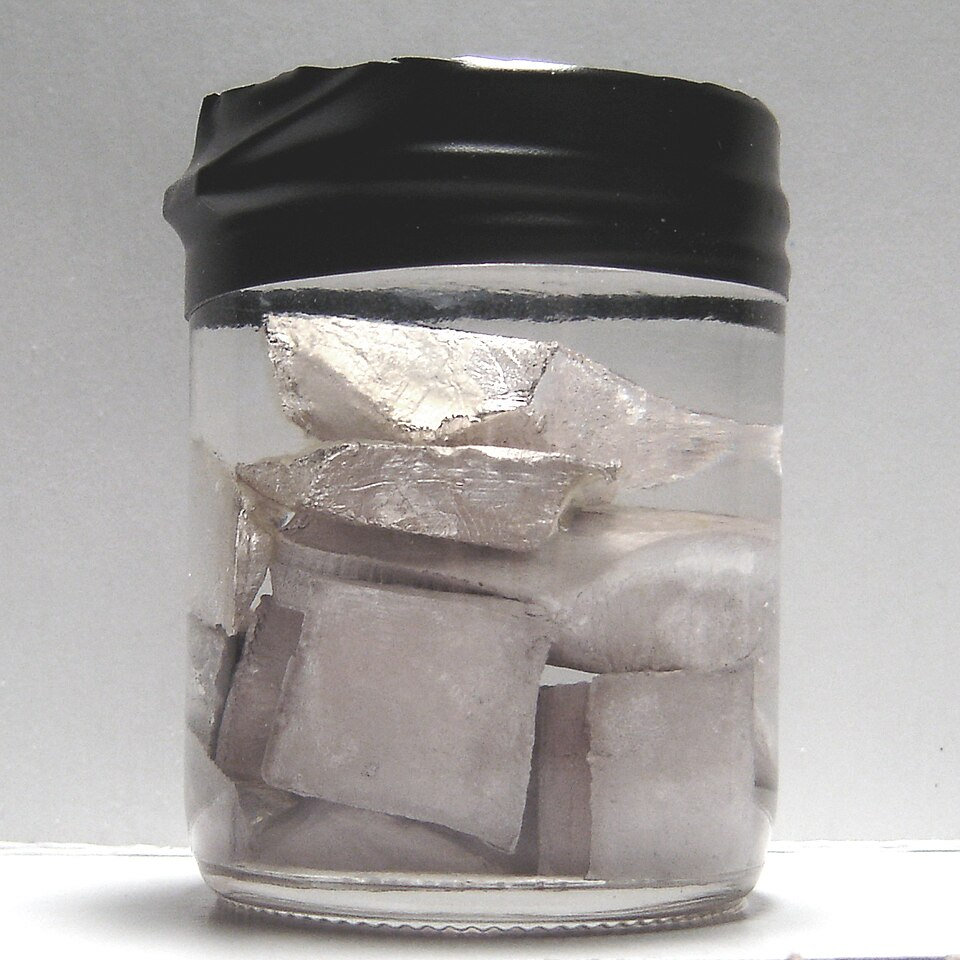
\includegraphics[height=4.6cm]{images/book2/sodium-oil.jpg}\hspace{0.8em}%
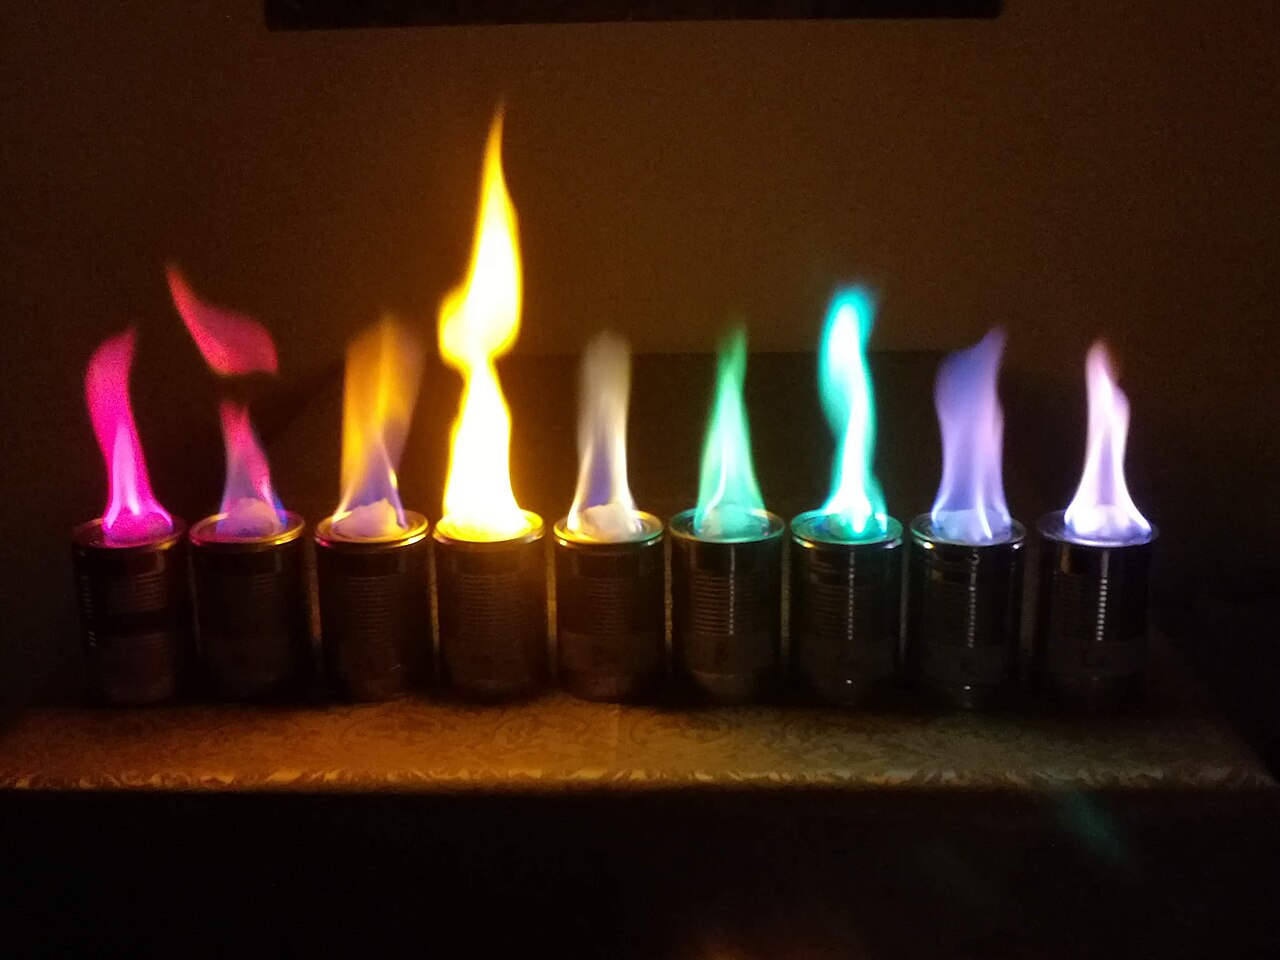
\includegraphics[height=4.6cm]{images/book2/flame-colours.jpg}

{\small बाएँ: सोडियम को वायु और नमी से दूर, खनिज तेल के नीचे रखा जाता है
(छायाचित्र: जस्टिन अर्जिटिस, CC BY-SA 2.5)। दाएँ: ज्वाला-रंग, बाएँ
से दाएँ, लिथियम, स्ट्रॉन्शियम, कैल्सियम, सोडियम, बेरियम, बोरॉन, कॉपर,
सीज़ियम और पोटैशियम यौगिकों के: ज्वाला में उत्तेजित इलेक्ट्रॉन
निम्नतर स्तरों पर लौटते हुए हर तत्त्व के अभिलाक्षणिक तरंगदैर्घ्यों पर प्रकाश उत्सर्जित करते हैं
(\cref{ch:b1:quantum-numbers}) (छायाचित्र: हेगलरास्ट, CC BY-SA 4.0)। दोनों
विकिमीडिया कॉमन्स।}
\end{omfigure}

\begin{inthelab}[एक प्रदर्शन, प्रयोग नहीं]
जल के साथ सोडियम की अभिक्रिया केवल शिक्षक द्वारा, सुरक्षा
पर्दे के पीछे, दिखाई जाती है: मसूर के दाने जितना टुकड़ा फ़िनॉल्फ़्थेलीन युक्त जल के
एक बड़े पात्र में डाला जाता है: धातु पिघलकर एक दौड़ती
गेंद बन जाती है, हाइड्रोजन सनसनाती है, और गुलाबी लकीर बने हाइड्रॉक्साइड को
दिखाती है। पोटैशियम हाइड्रोजन को प्रज्वलित कर देता है। बड़े टुकड़े विस्फोट करते हैं। सोडियम को
तेल के नीचे काटा जाता है, चिमटी से संभाला जाता है, और उसके अवशेष
एथेनॉल से नष्ट किए जाते हैं, कभी जल से नहीं।
\end{inthelab}

लिथियम अपने समूह का अपवाद है: सबसे छोटा आयन, सबसे
प्रबलता से जलयोजित, इसलिए सबसे ऋणात्मक विभव, फिर भी जल से
सबसे धीरे अभिक्रिया करने वाला। उसके यौगिक मैग्नीशियम के यौगिकों से मिलते-जुलते हैं (लिथियम
कार्बोनेट और फ़ॉस्फ़ेट अल्प विलेय हैं, जैसे मैग्नीशियम के), जो आवर्त सारणी में
एक विकर्ण संबंध है। \omterm{def:b1:s-block:families}{क्षार धातुएँ}
अपने गलित क्लोराइडों के विद्युत-अपघटन से बनाई जाती हैं, क्योंकि कोई भी रासायनिक
\omterm{def:b1:nernst:couple}{अपचायक} पर्याप्त प्रबल नहीं है; ऐसे सेलों की इलेक्ट्रोड अभिक्रियाओं का
अध्ययन द्वितीय वर्ष के खंड में है।

\section{उद्योग में सोडियम यौगिक}

\begin{definition}[ऑक्साइडों का स्वभाव]\label{def:b1:s-block:oxide-character}
\emph{क्षारकीय ऑक्साइड}\index{क्षारकीय ऑक्साइड} जल से अभिक्रिया करके
हाइड्रॉक्साइड देता है, या अम्लों से लवण (\ce{Na2O}, \ce{CaO}); \emph{अम्लीय
ऑक्साइड}\index{अम्लीय ऑक्साइड} जल से अभिक्रिया करके अम्ल देता है,
या क्षारकों से लवण (\ce{CO2}, \ce{SO3}, \ce{P4O10}); \emph{उभयधर्मी
ऑक्साइड}\index{उभयधर्मी ऑक्साइड} अम्लों और क्षारकों दोनों से अभिक्रिया करता है
(\ce{Al2O3}, \ce{ZnO})। किसी \omterm{def:b1:periodicity:table}{आवर्त} में आगे बढ़ने पर ऑक्साइड क्षारकीय
(धातुएँ, बाएँ) से अम्लीय (अधातुएँ, दाएँ) होते जाते हैं।
\end{definition}

सोडियम हाइड्रॉक्साइड लवण-जल के विद्युत-अपघटन से बनाया जाता है (क्लोर-क्षार
प्रक्रम, जो क्लोरीन और हाइड्रोजन भी देता है)। सोडियम कार्बोनेट, सोडा
ऐश, जो काँच, अपमार्जकों और लिथियम निष्कर्षण में प्रयुक्त होता है, या तो
ट्रोना खनिज के रूप में खोदा जाता है या लवण और चूना पत्थर से बनाया जाता है: 2025 में संसार ने
लगभग 7.1 करोड़ टन बनाया, 1.9 करोड़ प्राकृतिक निक्षेपों से और 5.2
करोड़ संश्लेषित, जिसका अधिकांश सॉल्वे प्रक्रम से।
% ledger: usgs:sodaash-total-2025, usgs:sodaash-natural-2025, usgs:sodaash-synthetic-2025

\begin{proposition}[सॉल्वे प्रक्रम]\label{prop:b1:s-block:solvay}
सॉल्वे प्रक्रम सोडियम क्लोराइड और कैल्सियम कार्बोनेट को
सोडियम कार्बोनेट और कैल्सियम क्लोराइड में बदलता है, \ce{2NaCl + CaCO3 -> Na2CO3 +
CaCl2}, ऐसे चरणों द्वारा जिनमें अमोनिया और कार्बन डाइऑक्साइड पुनःचक्रित होते हैं।
\end{proposition}

\begin{proof}
चरण ये हैं: (1) \ce{CaCO3 -> CaO + CO2} (भट्ठा); (2) \ce{NaCl + NH3 +
CO2 + H2O -> NaHCO3 + NH4Cl} (अमोनियायुक्त लवण-जल का कार्बोनेटन;
हाइड्रोजनकार्बोनेट, उपस्थित सबसे कम विलेय लवण, अवक्षेपित होता है); (3)
\ce{2NaHCO3 -> Na2CO3 + CO2 + H2O} (निस्तापन); (4) \ce{CaO + H2O ->
Ca(OH)2}; (5) \ce{Ca(OH)2 + 2NH4Cl -> CaCl2 + 2NH3 + 2H2O} (अमोनिया
पुनःप्राप्ति)। $(1) + 2\times(2) + (3) + (4) + (5)$ जोड़ने पर, \ce{NH3},
\ce{CO2}, \ce{NH4Cl}, \ce{NaHCO3}, \ce{CaO}, \ce{Ca(OH)2} और जल निरस्त हो जाते हैं:
\ce{2NaCl + CaCO3 -> Na2CO3 + CaCl2}।
\end{proof}

\begin{omfigure}
\begin{tikzpicture}[font=\small, >={Stealth}, box/.style={draw, rounded corners, fill=omDef!8, minimum width=2.6cm, minimum height=0.8cm, align=center}]
  \node[box] (kiln) at (0,0) {चूना भट्ठा\\\ce{CaCO3 -> CaO + CO2}};
  \node[box] (tower) at (5.3,0) {कार्बोनेटन मीनार\\\ce{NaHCO3} अवक्षेपित};
  \node[box] (calc) at (10.2,0) {निस्तापक\\\ce{NaHCO3} $\to$ \ce{Na2CO3}};
  \node[box] (slake) at (0,-2.6) {बुझाने का पात्र\\\ce{CaO + H2O -> Ca(OH)2}};
  \node[box] (still) at (5.3,-2.6) {अमोनिया आसवक\\\ce{NH4Cl + Ca(OH)2}};
  \draw[->, thick] (kiln) -- node[above] {\ce{CO2}} (tower);
  \draw[->, thick] (tower) -- node[above, font=\scriptsize] {\ce{NaHCO3}} (calc);
  \draw[->, thick] (calc.north) -- ++(0,0.6) -| node[pos=0.25, above] {\ce{CO2} पुनःचक्रित} (tower.north);
  \draw[->, thick] (kiln) -- node[left] {\ce{CaO}} (slake);
  \draw[->, thick] (slake) -- node[above, font=\scriptsize] {\ce{Ca(OH)2}} (still);
  \draw[->, thick] (tower) -- node[right] {\ce{NH4Cl}} (still);
  \draw[->, thick] (still.east) -- ++(1.2,0) |- node[pos=0.25, right] {\ce{NH3} पुनःचक्रित} ($(tower.east)+(0,-0.25)$);
  \draw[<-, thick] (tower.north west) -- ++(-0.5,0.6) node[above] {लवण-जल \ce{NaCl}};
  \draw[->, thick] (calc.east) -- ++(0.8,0) node[right] {\ce{Na2CO3}};
  \draw[->, thick] (still.south) -- ++(0,-0.6) node[below] {\ce{CaCl2}};
\end{tikzpicture}

{\small सॉल्वे प्रक्रम। कार्बन डाइऑक्साइड और अमोनिया चक्रों में घूमते हैं;
लवण और चूना पत्थर प्रवेश करते हैं, सोडा ऐश और कैल्सियम क्लोराइड निकलते हैं।}
\end{omfigure}

\begin{omfigure}
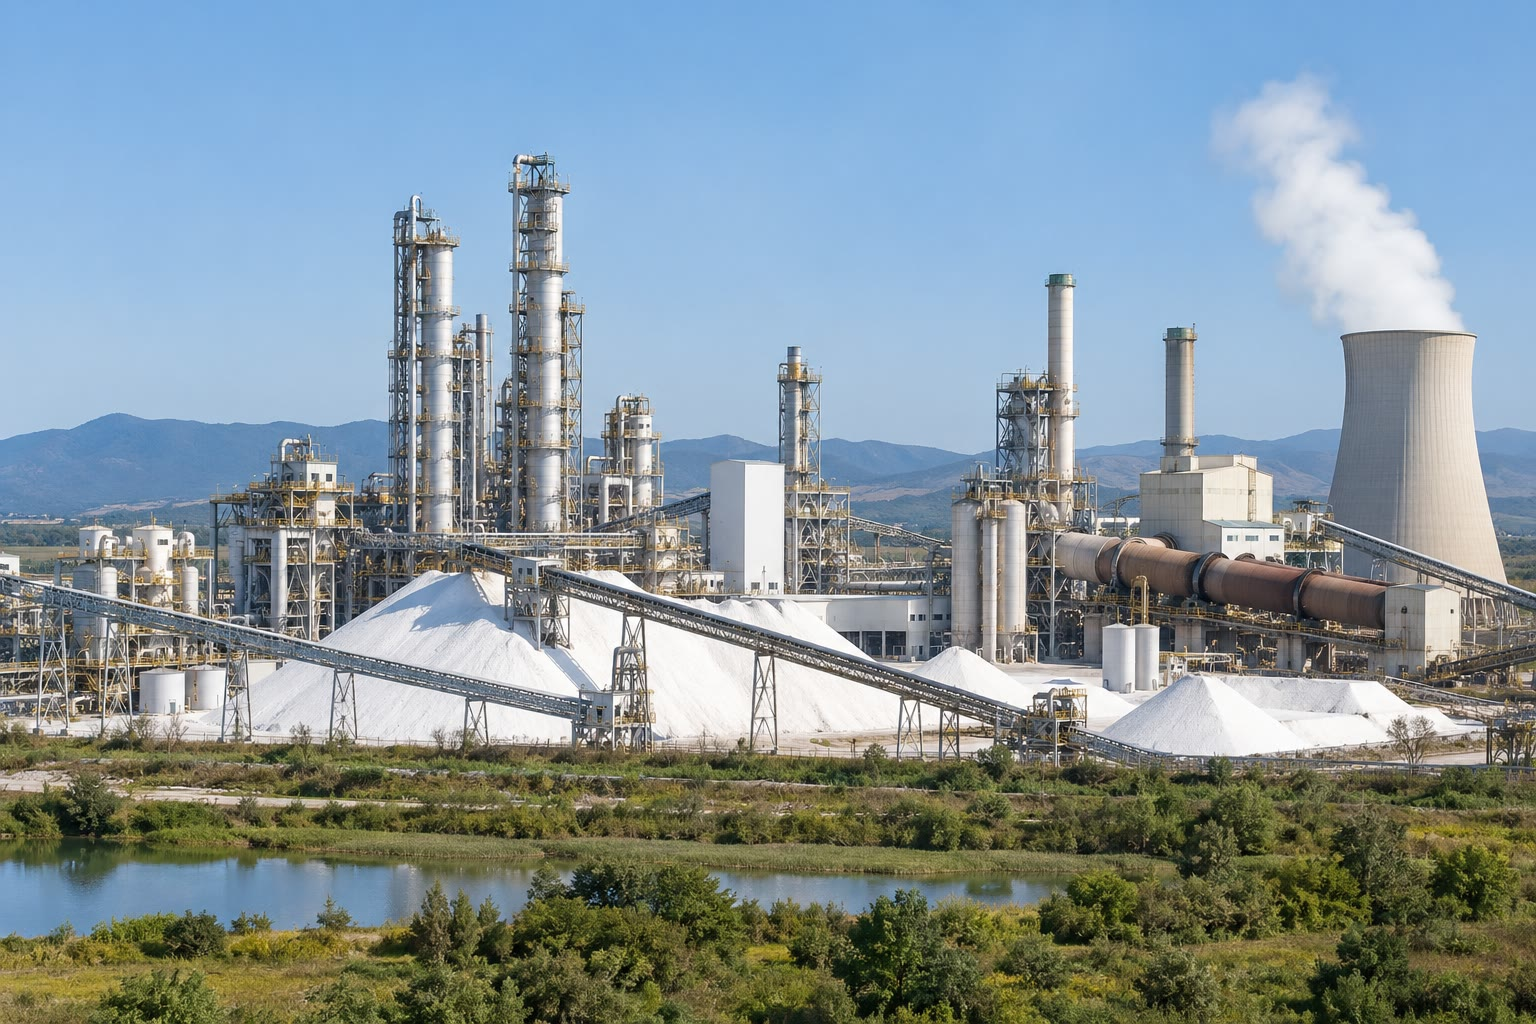
\includegraphics[width=0.55\linewidth]{images/book2/ai/b1-26-soda-ash-plant.jpg}

{\small एक सोडा-ऐश संयंत्र: चूना भट्ठे, कार्बोनेटन मीनारें और
सोडियम कार्बोनेट के ढेर।}
\end{omfigure}

\begin{method}[किसी प्रवाह-आरेख पर द्रव्यमान संतुलन]\label{met:b1:s-block:mass-balance}
\begin{enumerate}
  \item समग्र समीकरण लिखिए (चरणों का योग, पुनःचक्रित स्पीशीज़
        निरस्त)।
  \item वांछित उत्पाद से, समग्र समीकरण द्वारा कच्चे माल की मात्राएँ
        परिकलित कीजिए, फिर हर चरण की \omterm{def:b1:extent-q-and-k:fractional-extent}{लब्धि} के लिए संशोधन कीजिए।
  \item किसी पुनःचक्रित स्पीशीज़ के लिए केवल उतनी पूर्ति परिकलित कीजिए जो
        उसकी हानियों की भरपाई करे।
  \item निवेशों और निर्गमों के बीच हर तत्त्व के संतुलन की जाँच कीजिए।
\end{enumerate}
\end{method}

\section{क्षारीय मृदा धातुएँ}

मैग्नीशियम और कैल्सियम \omterm{def:b1:s-block:families}{क्षार धातुओं} से कम अभिक्रियाशील हैं (उच्चतर
आयनन ऊर्जाएँ: Mg \qty{7.65}{eV}, Ca 6.11; खोने के लिए दो इलेक्ट्रॉन) पर
फिर भी प्रबल \omterm{def:b1:nernst:couple}{अपचायक} हैं (\ce{Mg^2+}/\ce{Mg} का $E^\circ$ $-2.36$~V)।
मैग्नीशियम वायु में चकाचौंध करने वाले श्वेत प्रकाश के साथ जलता है; उसकी ऑक्साइड परत
कमरे के ताप पर उसकी रक्षा करती है। मैग्नीशियम समुद्री जल से
चूने द्वारा उसके हाइड्रॉक्साइड को अवक्षेपित करके प्राप्त किया जाता है, $\mathrm{p}K_s = 11.25$
(\cref{ch:b1:precipitation})।
% ledger: ie:Mg, ie:Ca

\begin{proposition}[चूना चक्र]\label{prop:b1:s-block:lime-cycle}
चूना पत्थर, बिना बुझा चूना, बुझा हुआ चूना और फिर चूना पत्थर एक चक्र बनाते हैं:
\ce{CaCO3 -> CaO + CO2} (भट्ठे में गरम करके); \ce{CaO + H2O -> Ca(OH)2}
(बुझाना, प्रबल ऊष्माक्षेपी); \ce{Ca(OH)2 + CO2 -> CaCO3 + H2O} (वायु में
चूने के गारे का जमना)। समग्र रूप से चक्र रासायनिक रूप से कुछ नहीं बदलता,
पर ऊर्जा और कार्बन डाइऑक्साइड का संचय और मोचन करता है।
\end{proposition}

\begin{proof}
तीनों समीकरण जोड़ने पर हर स्पीशीज़ निरस्त हो जाती है।
कार्बोनेट के अपघटन को ऊष्मा चाहिए, जो अन्य दो चरणों में फिर मुक्त होती है;
भट्ठे में निकली \ce{CO2} गारे द्वारा धीरे-धीरे फिर ग्रहण कर ली जाती है।
\end{proof}

\begin{omfigure}
\begin{tikzpicture}[font=\small, >={Stealth}]
  \node[draw, rounded corners, fill=omDef!8] (a) at (90:2.0) {\ce{CaCO3} चूना पत्थर};
  \node[draw, rounded corners, fill=omDef!8] (b) at (-30:2.0) {\ce{CaO} बिना बुझा चूना};
  \node[draw, rounded corners, fill=omDef!8] (c) at (210:2.0) {\ce{Ca(OH)2} बुझा हुआ चूना};
  \draw[->, thick] (a) to[bend left=25] node[right, align=left] {ऊष्मा\\$-\ce{CO2}$} (b);
  \draw[->, thick] (b) to[bend left=25] node[below] {$+\ce{H2O}$} (c);
  \draw[->, thick] (c) to[bend left=25] node[left, align=right] {$+\ce{CO2}$\\$-\ce{H2O}$} (a);
\end{tikzpicture}

{\small चूना चक्र, चूना पत्थर से गारे तक और वापस कैल्सियम
कार्बोनेट तक।}
\end{omfigure}

\section{लिथियम}

\begin{omfigure}
\begin{tikzpicture}
\begin{axis}[
  xbar, width=0.78\linewidth, height=5.4cm, xmin=0, xmax=110,
  symbolic y coords={CA,ML,BR,AR,ZW,CL,CN,AU}, ytick=data,
  yticklabels={कनाडा, माली, ब्राज़ील, अर्जेंटीना, ज़िम्बाब्वे, चिली, चीन, ऑस्ट्रेलिया},
  xlabel={2025 में खनित लिथियम (हज़ार टन Li, अनुमान)}, bar width=8pt,
  nodes near coords, every node near coord/.append style={font=\scriptsize},
  tick label style={font=\small}, label style={font=\small}, enlarge y limits=0.1]
\addplot[fill=omDef!45, draw=omDef] coordinates {(5.6,CA) (9.4,ML) (12,BR) (23,AR) (28,ZW) (56,CL) (62,CN) (92,AU)};
\end{axis}
\end{tikzpicture}

{\small 2025 में सबसे बड़े लिथियम उत्पादक (अनुमान; विश्व कुल
लगभग \num{290000} टन लिथियम)। ऑस्ट्रेलिया कठोर चट्टान
(स्पोड्यूमीन) खोदता है; चिली और अर्जेंटीना लवण-जल पंप करते हैं।}
% ledger: usgs:li-canada-2025, usgs:li-mali-2025, usgs:li-brazil-2025, usgs:li-argentina-2025, usgs:li-zimbabwe-2025, usgs:li-chile-2025, usgs:li-china-2025, usgs:li-australia-2025, usgs:li-world-2025
\end{omfigure}

लवण-जल को वाष्पन द्वारा सांद्र किया जाता है, चूने से मैग्नीशियम हटाया जाता है, और
सोडा ऐश से लिथियम कार्बोनेट अवक्षेपित किया जाता है। लिथियम कार्बोनेट का
असामान्य गुण है कि वह ठंडे की तुलना में गरम में कम विलेय है: \qty{20}{\celsius} पर
द्रव्यमान से \qty{1.31}{\percent}, \qty{80}{\celsius} पर \qty{0.84}{\percent},
\qty{100}{\celsius} पर \qty{0.71}{\percent}। इसलिए उसे
गरम विलयन से अवक्षेपित किया जाता है, जैसा सप्ताहांत समस्या परिकलित करती है।
% ledger: sol:Li2CO3-20, sol:Li2CO3-80, sol:Li2CO3-100

\section{अभ्यास}

\begin{exercise}[$\star$]\label{exo:b1:s-block:1}
लवणीय, सहसंयोजी या \omterm{def:b1:s-block:hydride}{धात्विक हाइड्राइड} के रूप में वर्गीकृत कीजिए: \ce{KH}, \ce{SiH4},
\ce{CaH2}, \ce{H2S}, \ce{PdH_{0.6}}। जल के साथ \ce{CaH2} की अभिक्रिया लिखिए।
\end{exercise}

\begin{exercise}[$\star$]\label{exo:b1:s-block:2}
जल के साथ लिथियम, सोडियम और पोटैशियम की, और तनु हाइड्रोक्लोरिक अम्ल के साथ
मैग्नीशियम की अभिक्रियाएँ लिखिए।
\end{exercise}

\begin{exercise}[$\star$]\label{exo:b1:s-block:3}
क्षारकीय, अम्लीय या उभयधर्मी के रूप में वर्गीकृत कीजिए: \ce{Na2O}, \ce{MgO}, \ce{Al2O3},
\ce{SiO2}, \ce{SO3}, \ce{ZnO}, \ce{CO2}। हर प्रकार के लिए एक अभिक्रिया लिखिए।
\end{exercise}

\begin{exercise}[$\star$]\label{exo:b1:s-block:4}
\omterm{def:b1:nernst:electrode-potential}{मानक विभवों} से pH 14 पर \ce{2Na + 2H2O -> 2Na+ + 2OH- + H2} का
स्थिरांक परिकलित कीजिए।
\end{exercise}

\begin{exercise}[$\star\star$]\label{exo:b1:s-block:5}
परमाणुओं के \omterm{def:b1:quantum-numbers:energy-level}{ऊर्जा स्तरों} (\cref{ch:b1:quantum-numbers}) का उपयोग करके लिथियम (लाल) और सोडियम (पीला)
के ज्वाला-रंगों की व्याख्या कीजिए। \qty{589}{nm} पर एक पीले फ़ोटॉन की ऊर्जा
क्या है?
\end{exercise}

\begin{exercise}[$\star\star$]\label{exo:b1:s-block:6}
\qty{90}{\percent} की समग्र \omterm{def:b1:extent-q-and-k:fractional-extent}{लब्धि} (सोडियम क्लोराइड के सापेक्ष) के साथ, सॉल्वे प्रक्रम द्वारा
एक टन सोडा ऐश के लिए आवश्यक चूना पत्थर (शुद्ध \ce{CaCO3}) और सोडियम क्लोराइड का
द्रव्यमान परिकलित कीजिए।
\end{exercise}

\begin{exercise}[$\star\star$]\label{exo:b1:s-block:7}
समुद्री जल में लगभग \qty{1.3}{g/L} मैग्नीशियम है (अभ्यास के
आँकड़े)। किस pH पर मैग्नीशियम हाइड्रॉक्साइड अवक्षेपित होना आरंभ होता है?
बुझे हुए चूने का कितना द्रव्यमान \qty{1.0}{m^3} के मैग्नीशियम को अवक्षेपित करता है?
\end{exercise}

\begin{exercise}[$\star\star$]\label{exo:b1:s-block:8}
लिथियम का \omterm{def:b1:nernst:electrode-potential}{मानक विभव} कम होने पर भी वह जल से पोटैशियम की तुलना में धीरे
अभिक्रिया क्यों करता है? ऊष्मागतिकी और गतिकी में भेद कीजिए।
\end{exercise}

\begin{exercise}[$\star\star$]\label{exo:b1:s-block:9}
एक टन चूना पत्थर से प्राप्त बिना बुझे चूने का द्रव्यमान और
\qty{25}{\celsius} तथा \qty{1}{bar} पर मुक्त \ce{CO2} का आयतन परिकलित कीजिए।
\end{exercise}

\begin{exercise}[$\star\star\star$]\label{exo:b1:s-block:10}
संसार ने 2025 में लगभग \num{290000} टन लिथियम खनित किया। यह कितने
लिथियम कार्बोनेट के बराबर है? यदि एक कार बैटरी में \qty{8}{kg}
लिथियम हो (अभ्यास के आँकड़े), तो यह कितनी बैटरियों की पूर्ति कर सकता है?
\end{exercise}

\begin{exercise}[$\star\star\star$]\label{exo:b1:s-block:11}
अध्याय के आँकड़ों से दिखाइए कि लिथियम कार्बोनेट की \omterm{def:b1:precipitation:solubility}{विलेयता} ताप के साथ घटती है,
और समझाइए कि उसे गरम अवस्था में अवक्षेपित करने से
लवण-जल से पुनःप्राप्ति क्यों सुधरती है।
\end{exercise}

\begin{exercise}[$\star\star\star$]\label{exo:b1:s-block:12}
सॉल्वे प्रक्रम के चरण (2) में विलयन में \ce{Na+},
\ce{NH4+}, \ce{Cl-} और \ce{HCO3-} हैं। समझाइए कि अमोनियम क्लोराइड के बजाय सोडियम हाइड्रोजनकार्बोनेट
क्यों अवक्षेपित होता है, और प्रक्रम को सोडियम हाइड्रॉक्साइड के बजाय
अमोनिया क्यों चाहिए।
\end{exercise}

\section{समस्या: लवण-जल से लिथियम}

\begin{problem}[{सप्ताहांत समस्या --- लिथियम लवण-जल को सांद्र करना,
चूने से मैग्नीशियम हटाना, सोडा
ऐश से लिथियम कार्बोनेट अवक्षेपित करना, और एक घन मीटर से पुनःप्राप्त लिथियम कार्बोनेट का द्रव्यमान}]
\label{pb:b1:s-block:1}
लवण-मैदान के नीचे से पंप किए गए लवण-जल में \qty{1.5}{g/L} लिथियम
और \qty{0.60}{g/L} मैग्नीशियम है (आयनों के रूप में, बहुत अधिक सोडियम क्लोराइड के साथ)।
तालाबों में वाष्पन उसे चार गुना सांद्र कर देता है। फिर सांद्र लवण-जल के
एक घन मीटर का उपचार किया जाता है: चूना मैग्नीशियम हटाता है, सोडा ऐश
कैल्सियम, और अंत में गरम सोडा ऐश \qty{80}{\celsius} पर लिथियम कार्बोनेट अवक्षेपित करता है।
आँकड़े: मोलर द्रव्यमान (\unit{g/mol}) Li 6.9, Mg 24.3,
\ce{Ca(OH)2} 74.1, \ce{Na2CO3} 106.0, \ce{Li2CO3} 73.8; $\mathrm{p}K_s$
\ce{Mg(OH)2} 11.25, \ce{CaCO3} 8.30; $\mathrm{p}K_e = 14.00$; \qty{80}{\celsius} पर
\ce{Li2CO3} की \omterm{def:b1:precipitation:solubility}{विलेयता} द्रव्यमान से \qty{0.84}{\percent}; अंतिम
मातृद्रव को \qty{1.0}{kg/L} घनत्व वाला \qty{1.00}{m^3} मानिए।

\medskip
\noindent\textbf{भाग I --- सांद्रण।}
\begin{enumerate}
  \item सांद्र लवण-जल में लिथियम और मैग्नीशियम की सांद्रताएँ
        परिकलित कीजिए।
  \item सांद्र लवण-जल के प्रति घन मीटर कितना आयतन जल
        वाष्पित होता है?
  \item गरम करने के बजाय सौर वाष्पन क्यों प्रयुक्त होता है?
  \item तालाबों में कौन-सा लवण सबसे पहले क्रिस्टलित होता है, और क्यों?
  \item एक घन मीटर में लिथियम और मैग्नीशियम की मात्राएँ परिकलित कीजिए।
  \item लिथियम के अवक्षेपण से पहले मैग्नीशियम को हटाना क्यों आवश्यक है?
\end{enumerate}

\medskip
\noindent\textbf{भाग II --- मैग्नीशियम और कैल्सियम हटाना।}
\begin{enumerate}[resume]
  \item बुझे हुए चूने के साथ मैग्नीशियम आयनों की अभिक्रिया लिखिए।
  \item आवश्यक बुझे हुए चूने का द्रव्यमान (रससमीकरणमितीय) परिकलित कीजिए।
  \item किस pH पर \qty{99.9}{\percent} मैग्नीशियम अवक्षेपित हो जाता है?
  \item लिथियम अपने हाइड्रॉक्साइड के रूप में अवक्षेपित क्यों नहीं होता?
  \item सोडा ऐश के साथ, लाए गए कैल्सियम का हटाया जाना लिखिए।
  \item उस चरण के लिए आवश्यक सोडा ऐश का द्रव्यमान परिकलित कीजिए।
\end{enumerate}

\medskip
\noindent\textbf{भाग III --- लिथियम कार्बोनेट।}
\begin{enumerate}[resume]
  \item लिथियम कार्बोनेट का अवक्षेपण लिखिए।
  \item लिथियम के लिए आवश्यक सोडा ऐश का द्रव्यमान परिकलित कीजिए।
  \item लिथियम कार्बोनेट का सैद्धांतिक द्रव्यमान परिकलित कीजिए।
  \item अवक्षेपण \qty{80}{\celsius} पर क्यों किया जाता है?
  \item लिथियम कार्बोनेट का कितना द्रव्यमान मातृद्रव में घुला रहता है?
  \item अवक्षेप को उसका अधिक भाग खोए बिना कैसे धोया जाता है?
\end{enumerate}

\medskip
\noindent\textbf{भाग IV --- संतुलन।}
\begin{enumerate}[resume]
  \item पुनःप्राप्त लिथियम कार्बोनेट का द्रव्यमान परिकलित कीजिए।
  \item लिथियम की पुनःप्राप्ति परिकलित कीजिए।
  \item सुझाइए कि मातृद्रव का क्या किया जाता है।
  \item एक घन मीटर में लिथियम की तुलना 2025 के विश्व उत्पादन
        से कीजिए: वह उत्पादन कितने घन मीटर के बराबर होगा?
  \item सांद्र लवण-जल के प्रति घन मीटर पुनःप्राप्त लिथियम कार्बोनेट का द्रव्यमान
        बताइए।
\end{enumerate}
\end{problem}
